\documentclass[9pt,xcolor=pdftex,dvipsnames,table]{beamer} 
\setbeamercolor{bgcolor}{fg=white,bg=blue!100}
\mode<presentation>
{
  \usetheme{Darmstadt}
 \setbeamertemplate{navigation symbols}{}
  \setbeamercovered{transparent}
  \setbeamertemplate{footline}
{\rightline{\insertframenumber/\inserttotalframenumber}}
}

\def\newblock{}

\newenvironment{changemargin}[2]{% 
  \begin{list}{}{% 
    \setlength{\topsep}{0pt}% 
    \setlength{\leftmargin}{#1}% 
    \setlength{\rightmargin}{#2}% 
    \setlength{\listparindent}{\parindent}% 
    \setlength{\itemindent}{\parindent}% 
    \setlength{\parsep}{\parskip}% 
  }% 
  \item[]}{\end{list}} 
  
\usepackage[english]{babel}
\usepackage{amsmath}
\usepackage{lipsum}
\usepackage[latin1]{inputenc}
\usepackage{times}
\usepackage[latin1]{inputenc}
\usepackage{tipa}
\usepackage{color}
\usepackage{listings}
\usepackage{booktabs}
\usepackage{colortbl}
\usepackage{movie15}
\usepackage{gb4e}
\usepackage{longtable}
\usepackage{pgf,pgfarrows,pgfnodes}
\usepackage{tikz} 
\usepackage{textpos}            % free image positioning 
\setlength{\TPVertModule}{1cm}  % unit for vertical positioning 
\setlength{\TPHorizModule}{1cm} % unit for horizontal positioning 

\definecolor{lightorange}{rgb}{1,0.75,.25}
\definecolor{lightred}{rgb}{1,0.25,.25}
\definecolor{lightblue}{rgb}{.25,.25,1.0}
\definecolor{lightgray}{rgb}{.75,.75,.75}

\usepackage[T1]{fontenc}

\title{Part of Speech Tagging}
\subtitle{}
\author{Linguistics 409 $\cdot$ Computational Linguistics}
\institute{Rice University}
\date[]{{\small \today}}
\usepackage{gb4e}

\usepackage{natbib}
\bibliographystyle{apalike}

\makeatletter
\newcommand\textsubscript[1]{\@textsubscript{\selectfont#1}}
\def\@textsubscript#1{{\m@th\ensuremath{_{\mbox{\fontsize\sf@size\z@#1}}}}}
\newcommand\textbothscript[2]{%
  \@textbothscript{\selectfont#1}{\selectfont#2}}
\def\@textbothscript#1#2{%
  {\m@th\ensuremath{%
    ^{\mbox{\fontsize\sf@size\z@#1}}%
    _{\mbox{\fontsize\sf@size\z@#2}}}}}
\def\@super{^}\def\@sub{_}
\makeatother

\begin{document}
\definecolor{grey}{rgb}{1,0.6,.7}

\section{Parts of Speech}

\begin{frame}

	\titlepage
	\begin{center}
		
\includegraphics[width=.2\paperwidth]{conjunction-junction.jpg}	
	\end{center}
\end{frame}

\subsection{}
\begin{frame}{Coming up...}
    \setbeamercovered{invisible}

	\begin{itemize}
		\item Today: Parts of Speech and Tagsets
		\item Monday: Tagging
	\end{itemize}
\end{frame}

\subsection{}
\begin{frame}{POS}

{\large 8 (ish) traditional parts of speech}
\vspace{.5cm}
\begin{itemize}
	\item Noun, verb, adjective, preposition, adverb, article, interjection, pronoun, conjunction, etc
	\item Called: parts-of-speech, lexical categories, word classes, morphological classes, lexical tags...
	\item Lots of debate within linguistics about the number, nature, and universality of these.  We'll completely ignore this debate.
\end{itemize}
\end{frame}

\subsection{}
\begin{frame}{Examples}
\begin{description}
	\item[N] (noun) chair, bandwidth, pacing
	\item[V] (verb) study, debate, munch
	\item[ADJ] (adjective) purple, tall, ridiculous
	\item[ADV] (adverb) unfortunately, slowly
	\item[P] (preposition) of, by, to
	\item[PRO] (pronoun) I, me, mine
	\item[DET] (determiner) the, a, that, those
\end{description}
\end{frame}

\subsection{}
\begin{frame}{Semantic descriptions fail.}

	\begin{center}
		{We typically try to define these (i.e. for children) semantically (see Schoolhouse Rock) but these descriptions ultimately fail.}
	\end{center}
\end{frame}

\subsection{}
\begin{frame}{Semantic descriptions fail.}

	{A better description is a \textbf{functional} or \textbf{distributional} account:}\\
	\vspace{.5cm}
	{\huge You shall know a word by the company it keeps}\\Firth, J. R. (1957:11)
\end{frame}



\subsection{}
\begin{frame}{Ambiguity}
	\begin{center}
		{\huge \textbf{entrance}}
	\end{center}
\end{frame}

\subsection{}
\begin{frame}{Ambiguity}
	\begin{center}
		{\huge She tended to \textbf{entrance} her visitors.}
	\end{center}
\end{frame}

\subsection{}
\begin{frame}{Ambiguity}
	\begin{center}
		{\huge \textbf{number}}
	\end{center}
\end{frame}

\subsection{}
\begin{frame}{Ambiguity}
	\begin{center}
		{\huge My fingers grew \textbf{number} the higher we climbed.}
	\end{center}
\end{frame}

\subsection{}
\begin{frame}{Ambiguity}
	\begin{center}
		{\huge \textbf{content}}
	\end{center}
\end{frame}

\subsection{}
\begin{frame}{Ambiguity}
	\begin{center}
		{\huge Despite the cost, \textbf{content} was scarce.}
	\end{center}
\end{frame}

\subsection{}
\begin{frame}{Coca Corpus}
	\begin{itemize}
		\item \url{http://corpus.byu.edu/coca/}
		\item \url{http://corpus.byu.edu/bnc/help/pos_c7.asp}
	\end{itemize}
\end{frame}

\subsection{}
\begin{frame}{Brown Corpus}
	\begin{itemize}
		\item \url{http://archive.org/details/BrownCorpus}
		\item \url{http://www.comp.leeds.ac.uk/ccalas/tagsets/brown.html}
	\end{itemize}
\end{frame}

\subsection{}
\begin{frame}{For next time:}

     \begin{block}{For next time:}
          \begin{enumerate}
          \item Monday: \textbf{Part of speech tagging}
          \item \textbf{Read:} J\&M chapter 5 pp 139 - 149
          \end{enumerate}
     \end{block}
\end{frame}

\subsection{}
\begin{frame}{Brown Corpus}
	\begin{itemize}
		\item \url{http://archive.org/details/BrownCorpus}
		\item \url{http://www.comp.leeds.ac.uk/ccalas/tagsets/brown.html}
	\end{itemize}
\end{frame}

\subsection{}
\begin{frame}{Two Basic Approaches to POS Tagging}
	\begin{itemize}
		\item Rule-based tagging (e.g. \href{http://www2.lingsoft.fi/cgi-bin/engtwol}{ENGTWOL})
		\vspace{.25cm}
		\item Machine learning approaches (stochastic tagging)
			\begin{itemize}
				\item HMM (Hidden Markov Model) tagging
				\item MEMMs (Maximum Entropy Markov Models)
			\end{itemize}
	\end{itemize}
\end{frame}

\section{Rule-Based Tagging}

\subsection{}
\begin{frame}{Rule-Based Tagging}

	\begin{itemize}
		\item Start with a dictionary
		\item Write rules by hand to selectively remove tags
		\item Leaving the correct tag for each word.
	\end{itemize}
\end{frame}

\subsection{}
\begin{frame}{Start with a dictionary...}

	\begin{description}
		\item[a] $<$Indef$>$ DET CENTRAL ART SG @DN$>$
		\item[aardvark] N NOM SG 
		\item[abaci] $<$?$>$ N NOM SG
		\item[aback] ADV
		\item[abacus] N NOM SG 
		\item[abaft] $<$?$>$ N NOM SG
		\item[abalone] $<$?$>$ N NOM SG
		\item[abandon] \begin{quote} $<$Indef> N NOM SG\\
	$<$SVO> V PRES -SG3 VFIN @+FMAINV\\
	$<$SVO> V INF\\
	$<$SVO> V IMP VFIN @+FMAINV\\
	$<$SVO> V SUBJUNCTIVE VFIN @+FMAINV\end{quote}
		\item[...]
	\end{description}
\end{frame}

\subsection{}
\begin{frame}{Assign all possible tags to each word}

\begin{center}

\begin{tabular}{l l l l l l}
     &          &      & V-SUBJ &     & V-SUBJ \\
     &          &      & V-INF  &     & V-IMF \\
     &          &      & V-IMP  &     & V-IMP \\
     & PCP2     & PREP & V-PRES &     & V-PRES \\
PRON & V-PAST   & TO   & N-SQ   & DET & N-SG \\\hline
She  & promised & to   & back   & the & bill\\
\end{tabular}
\end{center}
\end{frame}

\subsection{}
\begin{frame}{Write rules by hand to selectively remove tags}

\begin{center}
{\large \textbf{Eliminate PCP2 if V-PAST is an option when\\PCP2|V-PAST follows: <start> PRON}}

\vspace{.5cm}

\begin{tabular}{l l l l l l}
     &          &      & V-SUBJ &     & V-SUBJ \\
     &          &      & V-INF  &     & V-IMF \\
     &          &      & V-IMP  &     & V-IMP \\
     & \textbf{PCP2}     & PREP & V-PRES &     & V-PRES \\
PRON & V-PAST   & TO   & N-SQ   & DET & N-SG \\\hline
She  & promised & to   & back   & the & bill\\
\end{tabular}
\end{center}
\end{frame}

\subsection{}
\begin{frame}{Example: ENGTWOL (Stage 1)}

	\begin{itemize}
		\item First Stage: Run words through FST morphological analyzer to get all parts of speech.
		\item Example: Pavlov had shown that salivation ...
	\end{itemize}
	
	\vspace{.25cm}
	
	\begin{description}
		\item[Pavlov] PAVLOV N NOM SG PROPER
		\item[had] HAVE V PAST VFIN SVO\\HAVE PCP2 SVO
		\item[shown] SHOW PCP2 SVOO SVO SV
		\item[that] ADV\\PRON DEM SG\\DET CENTRAL DEM SG\\CS
		\item[salivation] N NOM SG
	\end{description}
\end{frame}

\subsection{}
\begin{frame}[fragile]
\frametitle{Example: ENGTWOL (Stage 2)}

	\begin{itemize}
		\item Second Stage: Apply \textbf{negative} constraints (3,774 total)
		\item Example: adverbial \emph{that} rule
		\item Eliminates all readings of \emph{that} except the one in, e.g.:
		\item `It isn't that odd'
	\end{itemize}
	
	\vspace{.25cm}
\begin{lstlisting}
Given input: that
If
(+1 A/ADV/QUANT) ;if next word is adj/adv/quantifier

(+2 SENT-LIM) ; following which is E-O-S

(NOT -1 SVOC/A)	; and the previous word is not a
                ; verb like `consider' which
                ; allows adjective complements
                ; in `I consider that odd'
Then eliminate non-ADV tags
Else eliminate ADV
\end{lstlisting}
\end{frame}

\section{HMM Tagging}

\subsection{}
\begin{frame}{Hidden Markov Model Tagging}

	\begin{itemize}
		\item Using an HMM to do POS tagging is a special case of Bayesian inference.
		\item It is also related to the `noisy channel model' that forms the basis for ASR, OCR and MT (as we'll see later)
	\end{itemize}
\end{frame}

\begin{frame}{HMM Tagging}

	\begin{itemize}
		\item Finds the highest probability sequence of tags given a sequence of words (though not directly!)
		\item Looks a wicked lot like minimum edit distance, e.g.
		\item Requires a training corpus/corpora and test corpus/corpora
		\item No probabilities for words not in corpus. (smoothing)
		\item Training corpus may be different from test corpus. (beware overfitting)
		\item We proceed by dynamic programming
	\end{itemize}
\end{frame}

\begin{frame}{HMM Tagging}

	\begin{itemize}
		\item \textbf{Intuition:} Pick the most likely tag for each word.
		\item HMM Taggers choose tag sequence that maximizes this formula:
		
			\begin{equation*}P( word | tag ) x P( tag| previous\,n\,tags)\end{equation*}  
			
		\item Let $T = t_1,t_2,..., t_n$
		\item Let $W = w_1,w_2,..., w_n$
		\item Find POS tags that generate a sequence of words --look  for most probable sequence of \textbf{hidden} tags $T$ underlying the observed words $W$.
	\end{itemize}
\end{frame}

\subsection{}
\begin{frame}{(Recall) Multiplication Rule}

{\large Multiplication Rule}
\vspace{.25cm}

     \begin{description}
          \item[\textbf{In general:}] $P(e_1, e_2) = P(e_1) x P(e_2 | e_1)$
     \end{description}

\vspace{.25cm}

We can rewrite the multiplication rule as a general definition for conditional
probability of two events $e$ and $f$:
\vspace{.5cm}

{\large \textbf{Bayes' rule}}

\begin{equation*}
P(e|f) = \frac{P(e,f)}{P(f)} = \frac{P(e) x P(f|e)}{P(f)}
\end{equation*}
\end{frame}

\begin{frame}{Bigram HMM Tagger}

	\begin{itemize}
		\item argmax P(T|W)
		\item argmax P(T)P(W|T)
		\item argmax P(t_1...t_n)P(w_1...w_n|t_1...t_n)
		\item argmax [P(t_1)P(t_2|t_1)...P(t_n|t_{n-1})][P(w_1|t_1)P(w_2|t_2)...P(w_n|t_n)]
	\end{itemize}
	\vspace{.25cm}
	
	{\large To tag a single word:} \begin{equation*}t_i = argmax P(t_i|t_{i-1})P(w_i|t_i)\end{equation*}

\end{frame}

\begin{frame}{Bigram HMM Tagger}

\begin{equation*}t_i = argmax P(t_i|t_{i-1})P(w_i|t_i)\end{equation*}

	\begin{itemize}
		\item How do we compute $P(t_i|t_{i-1})$?
			\begin{equation*}\frac{c(t_{i-1}t_i)}{c(t_{i-1})}\end{equation*}
		\item How do we compute $P(w_i|t_i)$?
			\begin{equation*}\frac{c(w_i,t_i)}{c(t_i)}\end{equation*}
		\item How do we compute the most probable tag sequence?
			\begin{equation*}Viterbi\end{equation*}
	\end{itemize}
\end{frame}

\section{Viterbi}

\begin{frame}{Viterbi Summary}

	\begin{itemize}
		\item Create a matrix
		\begin{itemize}
			\item Columns correspond to inputs
			\item Rows correspond to possible states
		\end{itemize}
		\item Sweep through the matrix in one pass filling the columns left to right using our transition probabilities and observations probabilities
		\item Key benefit of dynamic programming is that we need only store the MAX prob path to each cell (not the probabilities of all paths).
	\end{itemize}	
\end{frame}

\begin{frame}

	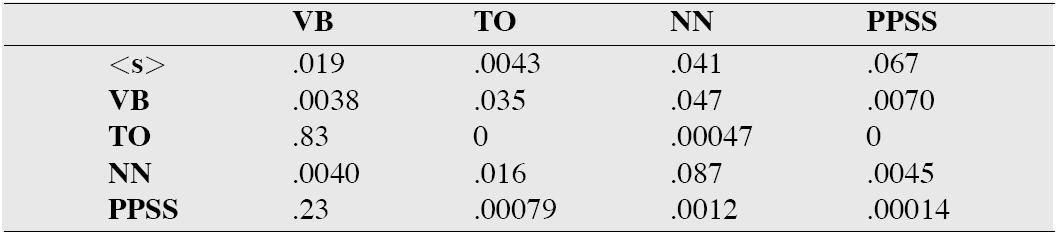
\includegraphics[width=.9\paperwidth]{hmmt1}\\
	\vspace{.5cm}
	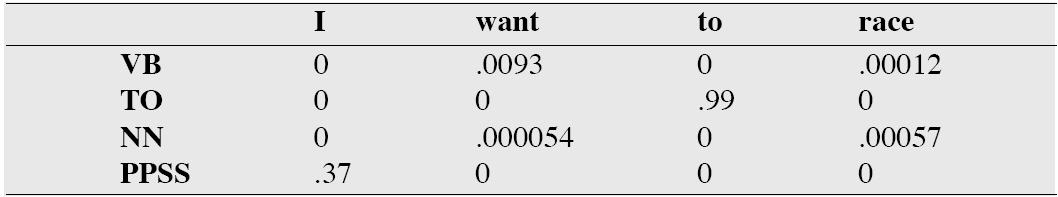
\includegraphics[width=.9\paperwidth]{hmmt2}	
\end{frame}

\begin{frame}{JM Figure 5.18: example Viterbi lattice}
	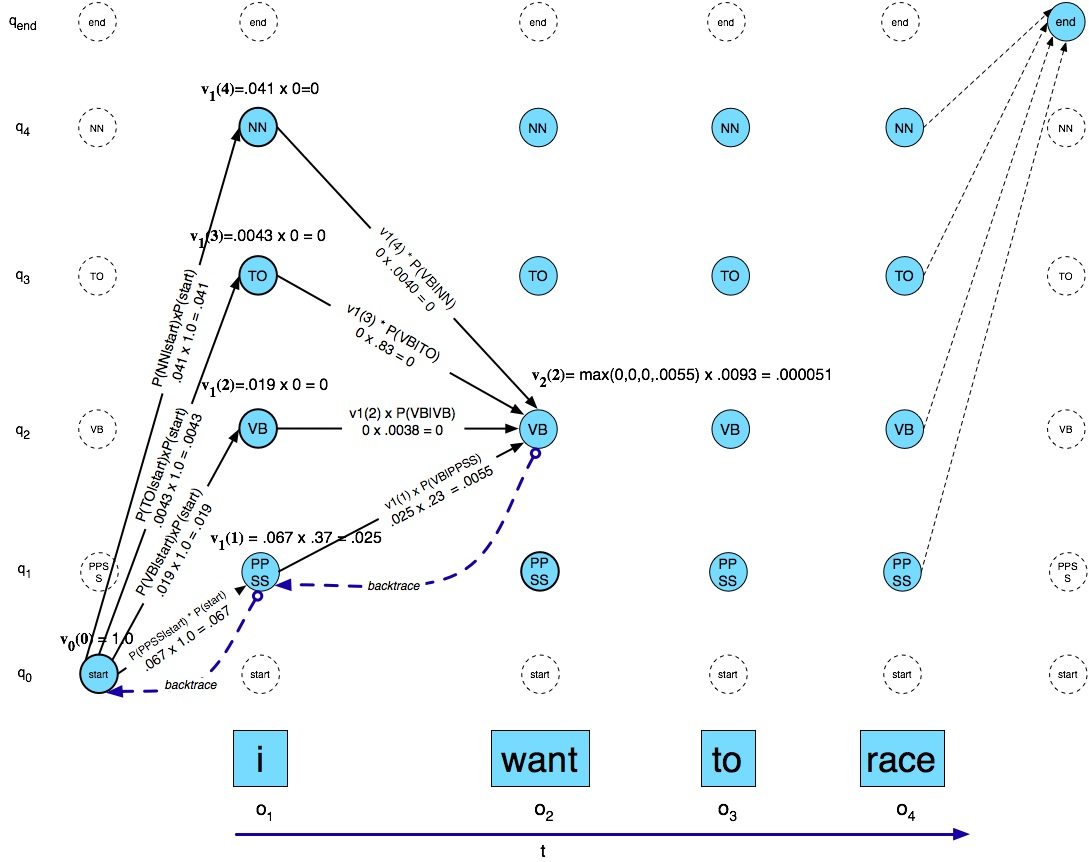
\includegraphics[width=.75\paperwidth]{pos5-18}
\end{frame}

\begin{frame}{Evaluation}

	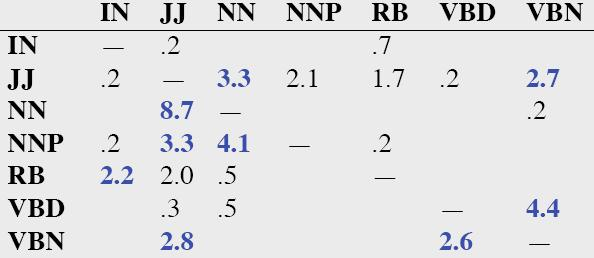
\includegraphics[width=.8\paperwidth]{hmm-confusion}\\
	\vspace{.5cm}
	\begin{itemize}
		\item Create a \textbf{confusion matrix}
		\item See which errors are most common and fix those.
		
		\begin{itemize}
			\item Noun (NN) vs ProperNoun (NNP) vs Adj (JJ)
			\item Preterite (VBD) vs Participle (VBN) vs Adjective (JJ)
		\end{itemize}
	\end{itemize}
\end{frame}

\begin{frame}{Evaluation}
	\begin{itemize}
		\item The result is compared with a manually coded ``Gold Standard''
		\item Typically accuracy reaches 96-97\%
		\item This may be compared with result for a baseline tagger (one that uses no context or less context).
		\item Important: 100\% is impossible even for human annotators!
	\end{itemize}
\end{frame}

\section{Brill}

\begin{frame}{Brill Taggers and Transformation Based Learning (TBL)}
	\begin{center}
		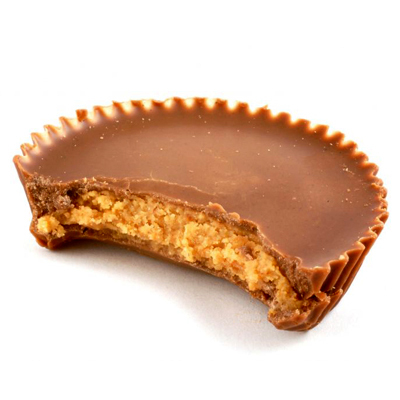
\includegraphics[width=.6\paperwidth]{reeses}
	\end{center}
\end{frame}

\begin{frame}{Rule-based vs. HMM-based taggers}

	\begin{enumerate}
		\item Rule-based taggers are nice because they capture a lot of explicit linguistic knowledge in a way that makes sense (and might be useable by other tools later in the pipeline).
		\item But they're expensive and slow to build and require a lot of human effort.
		\item HMM-based taggers, by contrast, require only a tagged corpus and are fast to train.
	\end{enumerate}
\end{frame}

\begin{frame}{Potential problems with HMM-based taggers}

{\large Brill (1995) identified two problems with HMM-based taggers:}
\vspace{.5cm}
	\begin{enumerate}
		\item ``stochastic taggers have the disadvantage that linguistic information is captured only indirectly, in large tables of statistics.''
		\item The relationships modelled by an HMM are between \textbf{tags} in a sequence and not between \textbf{words} in a sequence.
	\end{enumerate}
\end{frame}

\begin{frame}{Potential problems with HMM-based taggers}

{\large In HMM taggers,}

\vspace{.5cm}

\begin{itemize}
	\item ``state transition probabilities ($P(T_i | T_{i-1}... T_{i-n}$)) express the likelihood of a tag immediately following n other tags,
	\item and emit probabilities ($P(W_j | T_i)$) express the likelihood of a word, given a tag.
	\item Many useful relationships, such as that between a word and the previous word, or between a tag and the following word, are not directly captured by Markov-model based taggers.'' (Brill 1995, p. 555)
\end{itemize}
\end{frame}

\begin{frame}{Think about HMM-based taggers work...}
	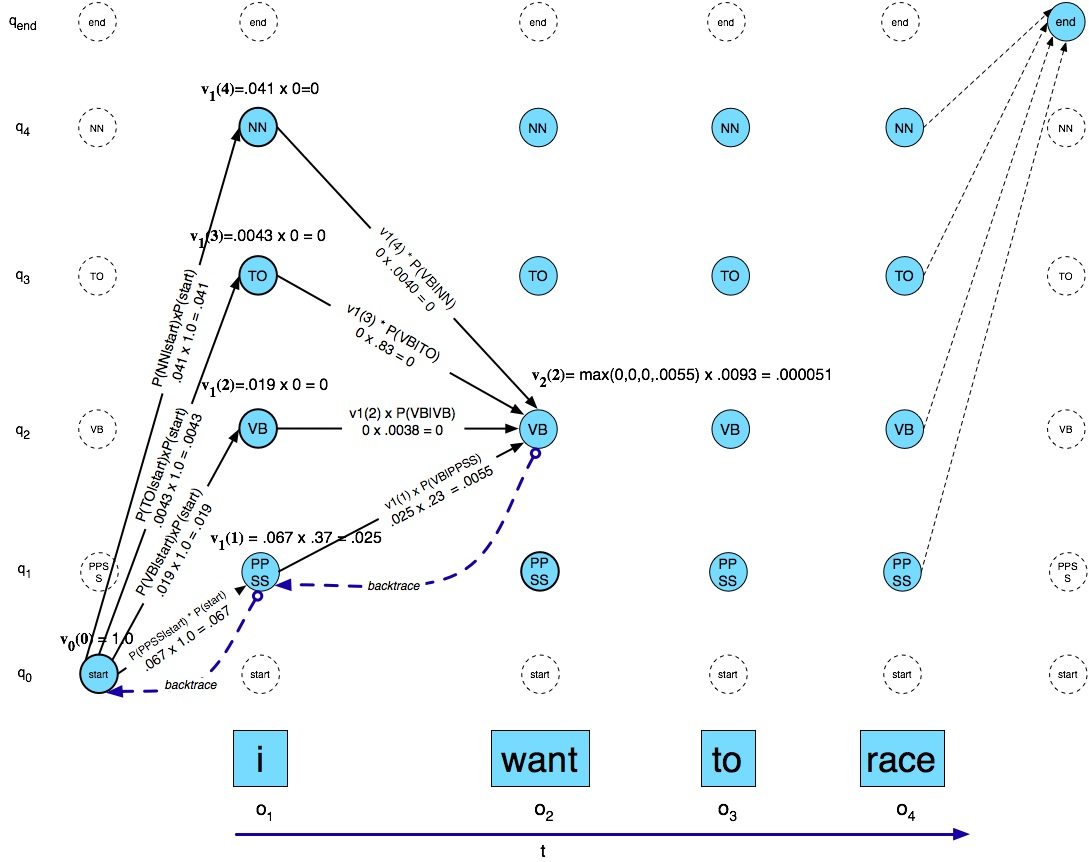
\includegraphics[width=.75\paperwidth]{pos5-18}
\end{frame}
		
\begin{frame}{Solution: Combine Them!}
	\begin{itemize}
		\item Use a simple stochastic (e.g. n-gram) tagger to provide an initial set of tags and then
		\item Apply a set of transformation rules to correct errors in these tag assignments.
		\item better still...
	\end{itemize}
\end{frame}

\begin{frame}{Solution: Combine Them!}

	\begin{center}
		{\large Don't write the rules by hand!  Learn them from a training corpus.}
	\end{center}
	\vspace{.5cm}
	\begin{enumerate}
		\item Assign most probable tag to each word (e.g. $P(DET|The)$) in a corpus.
		\item Compare automatic tag assignments to a hand-tagged version of that same corpus.
		\item Learn rules to correct the most frequent errors.
		\item Repeat 
	\end{enumerate}
\end{frame}

\begin{frame}{Machine Learning: three kinds of learning}

	\begin{description}
		\item[Supervised] Learn from entirely human-tagged data.
		\item[Unsupervised] Induce rules without recourse to human-tagged data.
		\item[Semi-Supervised] Bootstrap with human-tagged data, generalize to new data, retrain using both data sets.
	\end{description}
\end{frame}

\begin{frame}{Brill (1995) Example transformations learned from Penn Treebank}

	\begin{center}
		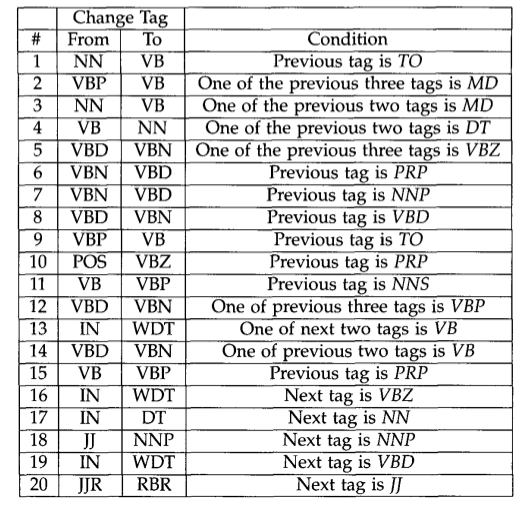
\includegraphics[width=.55\paperwidth]{brill3}\\
		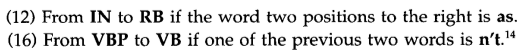
\includegraphics[width=.75\paperwidth]{brill4}
	\end{center}
\end{frame}

\begin{frame}{But how can it learn those rules?}

	\begin{center}
		{\large How must this work?\\How does the tagger know what kinds of relationships are possible between words and tags?}
	\end{center}
\end{frame}

\begin{frame}{Templates}

	{\large Templates specify the types of linguistic knowledge that can be learned from the data.  e.g.: \texttt{Change tag \textbf{a} to tag \textbf{b} when$\ldots$}}
	
	\begin{itemize}
		\item \texttt{$\ldots$ the (previous|next) tag is \textbf{z}}
		\item \texttt{$\ldots$ one of the (previous|next) two tags is \textbf{z}}
		\item \texttt{$\ldots$ one of the (previous|next) three tags is \textbf{z}}
		\item \texttt{$\ldots$ the (previous|next) word is \textbf{z}}
		\item \texttt{$\ldots$ the word three (before|after) is tagged \textbf{z}}
		\item \texttt{$\ldots$ the (previous|next) word is tagged \textbf{z} and the word two (before|after) is tagged \textbf{y}}
		\item etc.
	\end{itemize}
\end{frame}

\begin{frame}{Brill (1995) Figure 1: Error Driven Learning}

	\begin{center}
		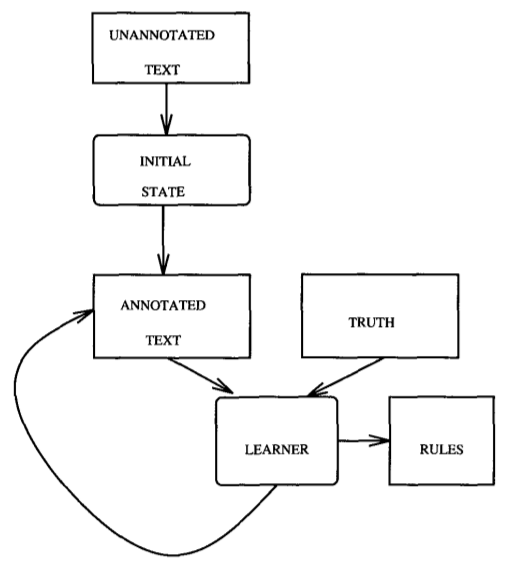
\includegraphics[width=.5\paperwidth]{brill1}
	\end{center}
\end{frame}

\begin{frame}{Brill (1995) Figure 2: Example Error Driven Learning}

	\begin{center}
		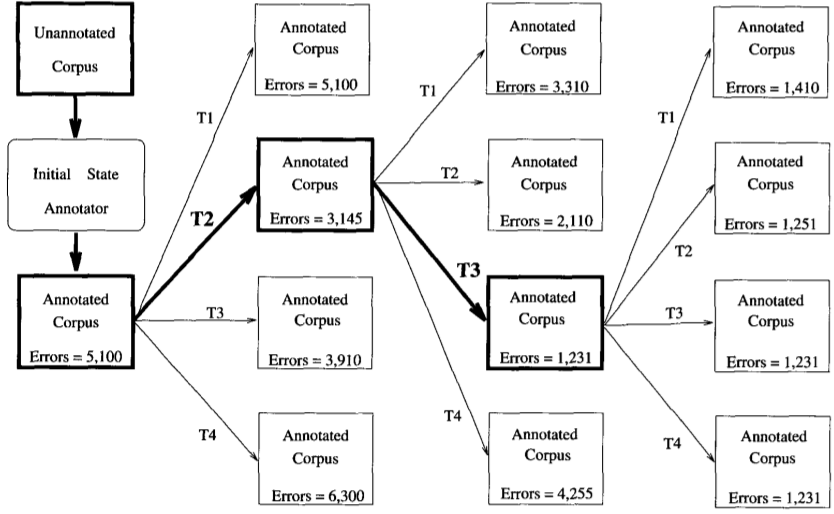
\includegraphics[width=.9\paperwidth]{brill2}
	\end{center}
\end{frame}

\begin{frame}{Brill Demonstration}

	\begin{center}
		{\large Brill demonstration using Python and NLTK }
	\end{center}
\end{frame}

\section{Conclusion}

\subsection{}
\begin{frame}{For next time:}

     \begin{block}{For next time:}
          \begin{enumerate}
          \item Friday: \textbf{Hidden Markov Models}
          \item \textbf{Read:} J\&M chapter 6 pp 173 - 183 
          \end{enumerate}
     \end{block}
\end{frame}

\end{document}
